% !TEX root = ../modelo-ifg.tex

\chapter{Referencial Teórico}
\label{cap:ref_teorico}

Para viabilizar uma arquitetura autônoma e de baixo custo voltada à detecção precoce de focos de
incêndio em áreas remotas de preservação utilizando modelos de Inteligência Artificial, torna-se
necessário discorrer sobre as diferentes tecnologias e técnicas que serão utilizadas para o
desenvolvimento do sistema.

% ============================================================
\section{Visão Computacional}
\label{sec:visao_computacional}
% ============================================================

Modelos de IA aplicados à Visão Computacional são amplamente empregados no reconhecimento de
padrões complexos em imagens. No âmbito dos modelos baseados em CNNs, um avanço decisivo ocorreu
com o desenvolvimento da arquitetura Faster R-CNN (Figura~\ref{fig:faster_rcnn}) por
\citeonline{ren2015faster}, que introduziu a \textit{Region Proposal Network} (RPN), integrando a
geração de propostas de regiões ao treinamento ponta a ponta e otimizando o tempo de
processamento, atingindo valores de 0,5 quadros por segundo (FPS).

\begin{figure}[htbp]
  \centering
  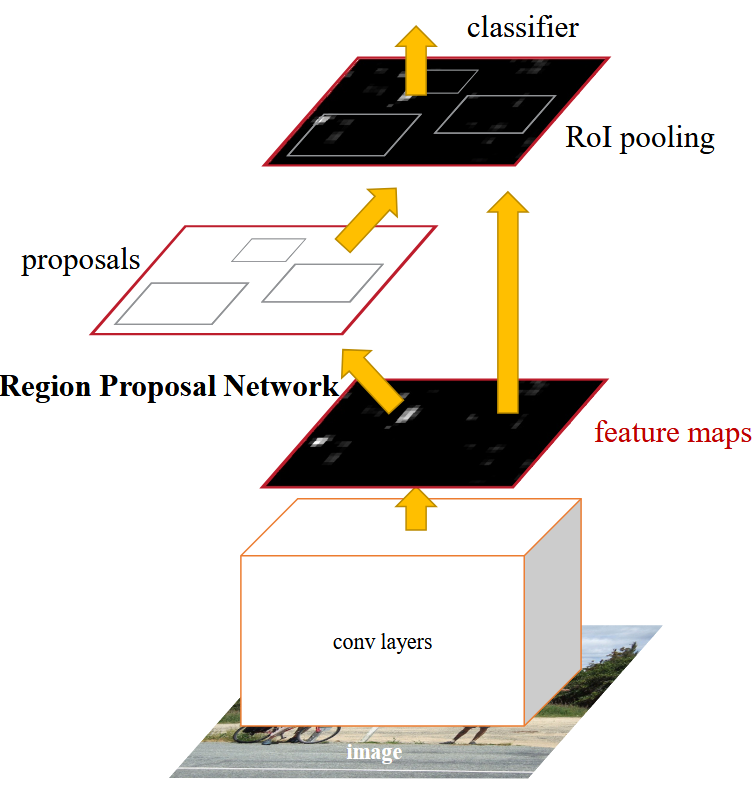
\includegraphics[width=0.40\textwidth]{fig/faster-rcnn}
  \caption{Arquitetura do modelo Faster R-CNN. O fluxo apresenta a extração de mapas de
  características por camadas convolucionais, seguida pela RPN, que atua direcionando a atenção
  da rede para a geração das propostas de regiões submetidas à camada de \textit{RoI Pooling} e
  ao classificador final.}
  \label{fig:faster_rcnn}
  \fontefig{Fonte: \citeonline{ren2015faster}}
\end{figure}

Posteriormente, \citeonline{redmon2016yolo} propuseram o YOLOv1 (\textit{You Only Look Once}).
A abordagem ilustrada pela Figura~\ref{fig:yolo_arch} redefiniu a tarefa ao estruturar a imagem em
uma grade regular e formular a predição das coordenadas das caixas delimitadoras
(\textit{Bounding Boxes}) e das probabilidades de classe como um problema único de regressão
direta. Essa arquitetura de CNN foi capaz de atingir o marco de 45 FPS processados em tempo real,
embora apresentasse limitações na localização de objetos pequenos e agrupados.

\citeonline{liu2016ssd} introduziu uma solução alternativa denominada \textit{Single Shot Multibox
Detector} (SSD). Enquanto o YOLO utilizava apenas o último mapa de características e dependia de
camadas densas no topo da rede, o SSD eliminou as camadas totalmente conectadas e formulou uma
estrutura puramente convolucional. Esse modelo, por sua vez, contornava o gargalo apresentado pelo
modelo YOLOv1 em detectar pequenas \textit{Bounding Boxes}, sendo necessário 1,6 giga de operações
de ponto flutuante (GFLOPS). Na Figura~\ref{fig:ssd_comparativo} é apresentada uma comparação
direta entre as arquiteturas desenvolvidas, além de trazer o comparativo de eficiência dos modelos.

Diante do aumento da demanda por processamento em dispositivos de borda, algumas restrições quanto
à complexidade computacional dos modelos CNNs foram impostas. Nesse cenário,
\citeonline{howard2017mobilenets} junto à equipe da Google apresentaram as Convoluções Separáveis
em Profundidade (\textit{Depthwise Separable Convolutions}) através do modelo MobileNet proposto.
A nova estrutura proposta do modelo CNN reduziu em aproximadamente 8 a 9 vezes os parâmetros e as
operações para 1,13 kFLOPs.

\begin{figure}[htbp]
  \centering
  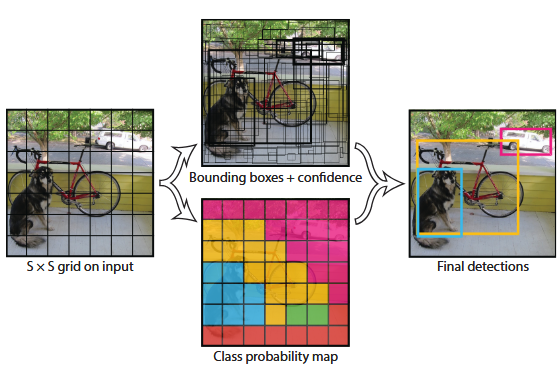
\includegraphics[width=0.60\textwidth]{fig/yolo-grid}
  \caption{Funcionamento da arquitetura da CNN YOLO. O sistema YOLO divide a imagem de entrada a
  partir de um grid de $S \times S$ e processa cada célula e prevê $B$ \textit{Bounding Boxes}
  para cada uma e $C$ probabilidade de classes.}
  \label{fig:yolo_arch}
  \fontefig{Fonte: \citeonline{ren2015faster}}
\end{figure}

\begin{figure}[htbp]
  \centering
  \caption{Comparativo de eficiência entre as arquiteturas Faster R-CNN, YOLO e SSD.}
  \label{fig:ssd_comparativo}
  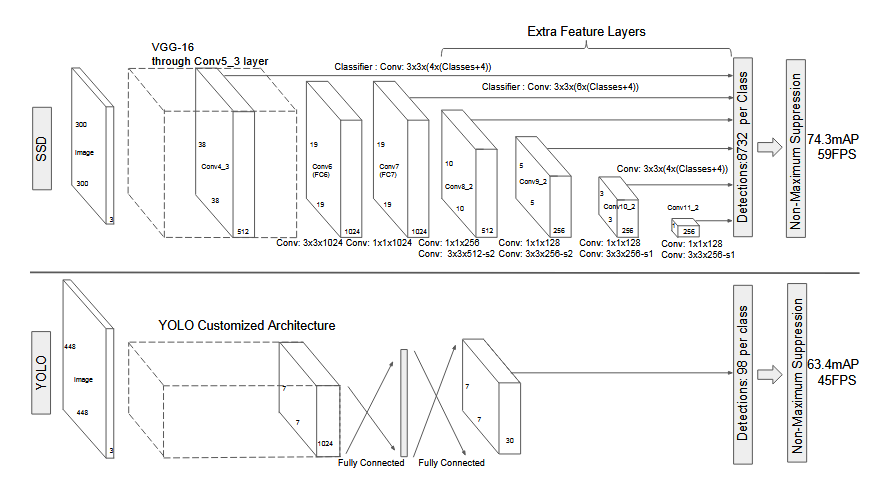
\includegraphics[width=0.85\textwidth]{fig/ssd-comparativo}
  \fontefig{Fonte: \citeonline{liu2016ssd}}
\end{figure}

O desenvolvimento de arquiteturas baseadas em CNNs evoluiu substancialmente, impulsionando o
surgimento de diversos modelos voltados para \textit{Edge AI}. Essas redes exploram diferentes
abordagens estruturais e técnicas de compressão computacional para maximizar a eficiência
energética e a velocidade de inferência. Tais tecnologias deverão ser analisadas em relação à
eficácia e custo computacional a fim de selecionar o modelo ideal para realizar a identificação e
a classificação de focos de incêndio.

% ============================================================
\section{Equipamentos de \textit{Edge AI}}
\label{sec:edge_ai}
% ============================================================

O avanço substancial do aprendizado profundo, impulsionado em 2012 pela vitória da AlexNet
\cite{krizhevsky2012imagenet} no desafio da \textit{ImageNet}, estabeleceu um ponto de inflexão na
área de visão computacional. Embora já existissem plataformas embarcadas capazes de processar
algoritmos clássicos de processamento de imagem, como a Raspberry Pi 1 Model~B
\cite{raspberrypi_modelb} apresentado na Figura~\ref{fig:raspberry_pi}, tais dispositivos
apresentavam severas limitações computacionais para suprir a elevada demanda de FLOPs exigida pelas
redes convolucionais profundas.

\begin{figure}[htbp]
  \centering
  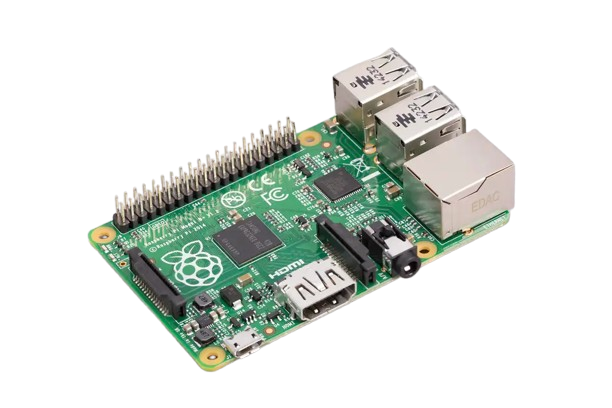
\includegraphics[width=0.60\textwidth]{fig/raspberry-pi}
  \caption{Dispositivo Raspberry Pi 1 Model B+, substituto do Model B anterior.}
  \label{fig:raspberry_pi}
  \fontefig{Fonte: Adaptado de \citeonline{raspberrypi_modelb}.}
\end{figure}

Para mitigar esse gargalo, a indústria de semicondutores voltou seus esforços ao desenvolvimento
de arquiteturas de hardware voltadas à aceleração dessas cargas de trabalho. Como marco dessa
transição, a NVIDIA introduziu em 2014 a placa Jetson TK1 \cite{harrys2014jetson}, que incorporou
núcleos CUDA ao ecossistema de sistemas embarcados. Essa convergência viabilizou a consolidação de
dispositivos modernos de \textit{Edge AI}, garantindo capacidade de processamento local, redução
crítica de latência e autonomia operacional para instalações remotas ou sujeitas a restrições de
conectividade de rede.

\begin{figure}[htbp]
  \centering
  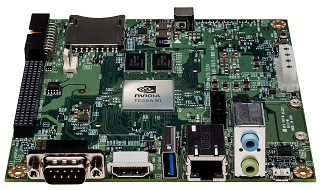
\includegraphics[width=0.45\textwidth]{fig/jetson-tk1}
  \caption{Dispositivo NVIDIA Jetson TK1.}
  \label{fig:jetson_tk1}
  \fontefig{Fonte: \citeonline{harrys2014jetson}}
\end{figure}

Nos anos subsequentes, o mercado testemunhou uma proliferação de plataformas orientadas a ampliar
a eficiência no processamento de tais algoritmos. Enquanto a NVIDIA expandia sua linha com
arquiteturas gráficas progressivamente mais potentes, outros fabricantes, a exemplo da Intel,
investiram no projeto de unidades de aceleração dedicadas. Nesse contexto, a Intel anunciou em
2017 a VPU Movidius Myriad X, incorporando o \textit{Neural Compute Engine} (NCE) -- um bloco de
hardware de função fixa projetado para a aceleração de operações convolucionais que elevou o
rendimento do chip para 1 trilhão de operações por segundo (TOPS) \cite{intel2018myriad}.

Em contrapartida, no ano de 2019, a Google estabeleceu um marco no setor ao introduzir a Edge TPU.
O circuito integrado baseava-se em uma matriz sistólica de multiplicação e acumulação
(\textit{Multiply-Accumulate} -- MAC) otimizada estritamente para o \textit{runtime} TensorFlow
Lite com tensores quantizados em INT8, alcançando 4 TOPS com consumo de apenas 2\,W. Desde então,
essas tecnologias vêm sendo continuamente aprimoradas por fabricantes consolidados e novos
concorrentes, mantendo a maximização da eficiência energética e do rendimento computacional no
centro do desenvolvimento de hardware para \textit{Edge AI}.

% ============================================================
\section{Câmeras de Monitoramento de Longo Alcance}
\label{sec:cameras}
% ============================================================

As câmeras de monitoramento modernas integram recursos ópticos e computacionais projetados para
maximizar a resolução, o alcance e a fidelidade visual das capturas, além de apresentar robustez
mecânica contra intempéries. Complementarmente, esses dispositivos incorporam funcionalidades
analíticas embarcadas, viabilizando a identificação e a classificação automática de eventos,
transeuntes, animais e objetos de interesse na cena vigiada.

Em termos de mobilidade física, as câmeras PTZ (\textit{Pan-Tilt-Zoom}) diferenciam-se por
integrar eixos motorizados para varredura horizontal (\textit{pan}) e ajuste vertical
(\textit{tilt}), aliados a lentes de zoom óptico ajustável. Essa configuração é essencial para o
monitoramento florestal e a detecção de incêndios, pois permite a cobertura contínua de grandes
extensões de área e a inspeção detalhada de fumaça a longas distâncias.

Contudo, tais recursos mecânicos e ópticos não bastam para mitigar todos os desafios inerentes à
detecção de queimadas. As limitações do sensoriamento restrito ao espectro da luz visível
permanecem como um obstáculo crítico, decorrentes tanto da ausência de irradiância solar durante o
período noturno quanto de atenuações atmosféricas severas provocadas por nevoeiros ou densas
colunas de fumaça. Para mitigar esses entraves, soluções modernas de sensoriamento empregam
sensores no espectro infravermelho (\textit{Infrared} -- IR), permitindo a detecção térmica
contínua independentemente da iluminação visível \cite{driggers2022introduction}. Conforme
apresentado na Figura~\ref{fig:espectro_ir}, a radiação infravermelha abrange cinco regiões
espectrais: o infravermelho próximo (NIR), o infravermelho de ondas curtas (SWIR), o infravermelho
de ondas médias (MWIR), o infravermelho de ondas longas (LWIR) e o infravermelho distante (FIR).

\begin{figure}[htbp]
  \centering
  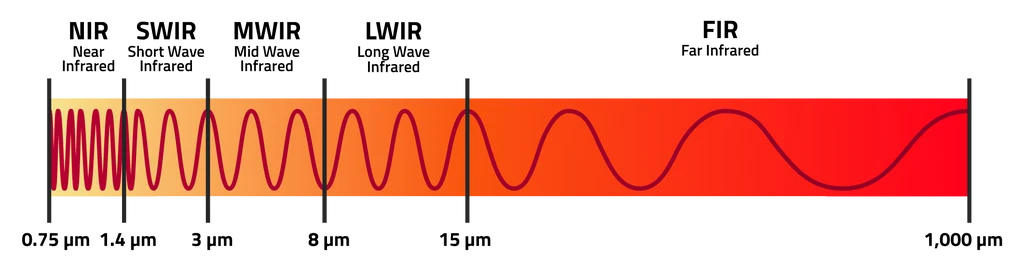
\includegraphics[width=\textwidth]{fig/espectro-infravermelho}
  \caption{Faixas do espectro eletromagnético infravermelho e seus respectivos intervalos de
  comprimento de onda ($\mu$m).}
  \label{fig:espectro_ir}
  \fontefig{Fonte: \citeonline{advexure2023thermal}}
\end{figure}

No contexto do monitoramento e detecção precoce de incêndios em áreas de preservação, cada banda
do espectro infravermelho desempenha funções analíticas distintas conforme as propriedades físicas
de emissão e propagação \cite{driggers2022introduction}:

\begin{description}
  \item[\textbf{NIR (0,75 -- 1,4\,$\mu$m):}] Opera predominantemente pela reflexão de luz (solar
  ou artificial de LEDs IR), viabilizando a vigilância noturna convencional e a avaliação da
  reflectância foliar para monitorar o ressecamento da biomassa florestal, embora ainda sofra
  bloqueio visual frente a fumaças espessas.

  \item[\textbf{SWIR (1,4 -- 3\,$\mu$m):}] Apresenta menor dispersão por aerossóis (espalhamento
  de Rayleigh e Mie), permitindo penetrar névoas e fumaças dispersas. Capta anomalias térmicas
  severas ($>$\,800\,K) sem a saturação precoce comum aos sensores do espectro visível.

  \item[\textbf{MWIR (3 -- 8\,$\mu$m):}] Coincide com o pico espectral de irradiância das frentes
  de combustão ativa (600\,K a 1.200\,K) ditado pela Lei de Wien. É a banda mais indicada para
  discriminar chamas ativas e identificar gases quentes oriundos da combustão.

  \item[\textbf{LWIR (8 -- 15\,$\mu$m):}] Coincide com a curva radiativa da superfície terrestre
  e da vegetação à temperatura ambiente ($\approx$300\,K), possibilitando operação passiva 24/7
  sem necessidade de iluminação externa, transpassando fumaça densa e revelando brasas
  subterrâneas, troncos incandescentes e rescaldo.

  \item[\textbf{FIR (15 -- 1.000\,$\mu$m):}] Correspondente a emissões térmicas de corpos
  extremamente frios, apresenta forte atenuação atmosférica na baixa troposfera devido à absorção
  molecular, o que limita seu emprego em câmeras ópticas de vigilância terrestre, restringindo seu
  uso majoritariamente a estudos climatológicos e astronômicos.
\end{description}

No entanto, a integração dessas faixas do infravermelho em câmeras de monitoramento esbarra em
restrições técnicas que aumentam o custo da tecnologia. A necessidade de materiais ópticos
especializados (como lentes de germânio, transparentes ao infravermelho médio e longo) somada à
suscetibilidade dos detectores térmicos ao ruído -- exigindo módulos de dissipação térmica ou
rotinas constantes de recalibração radiométrica -- eleva consideravelmente o custo de aquisição e
implantação desses dispositivos em campo.

% ============================================================
\section{Alimentação \textit{Off-Grid}}
\label{sec:alimentacao}
% ============================================================

Com o intuito de garantir a operação ininterrupta do sistema de forma autônoma e sem necessidade
de intervenção humana direta, a infraestrutura deve contar com um subsistema de alimentação
energética sustentável e autossuficiente. Ao avaliar as alternativas disponíveis para a
implementação desse subsistema em regiões isoladas, a geração solar fotovoltaica consolida-se
como a abordagem mais viável. Essa escolha fundamenta-se na elevada disponibilidade de irradiância
solar típica do bioma Cerrado, de acordo com a Figura~\ref{fig:atlas_solar}, aliada à ausência de
componentes móveis na conversão de energia, o que reduz substancialmente a demanda de manutenção
mecânica, mitiga o risco de falhas em campo e oferece uma relação custo-benefício superior quando
associada a um banco de baterias dimensionado para suprir períodos de baixa insolação ou operação
noturna contínua.

\begin{figure}[htbp]
  \centering
  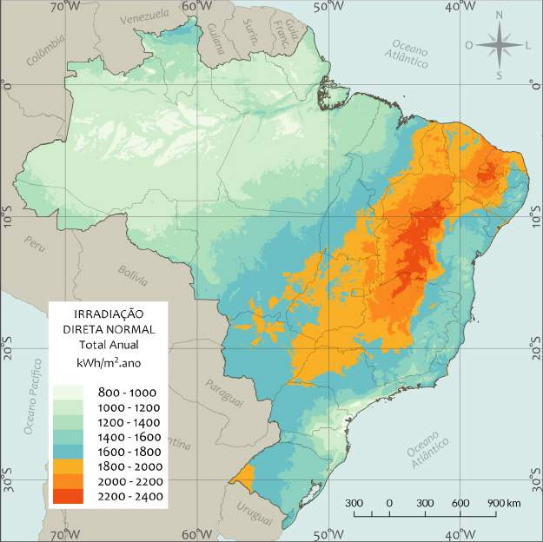
\includegraphics[width=0.65 \textwidth]{fig/atlas-solar}
  \caption{Mapa do total anual de irradiação solar direta normal com destaque para regiões com
  maior potencial de aproveitamento da energia solar concentrada.}
  \label{fig:atlas_solar}
  \fontefig{Fonte: \citeonline{pereira2017atlas}}
\end{figure}

A implementação prática dessa estrutura fotovoltaica autônoma demanda um arranjo integrado por
módulos de geração, controle, armazenamento e conversão de energia. Nesse contexto, o controlador
de carga atua na regulação da tensão e da corrente provenientes dos painéis fotovoltaicos,
gerenciando os ciclos de recarga e prevenindo sobrecargas ou descargas profundas no acumulador.
O armazenamento energético apoia-se em um banco de baterias estacionárias de ciclo profundo,
responsável por assegurar o suprimento ininterrupto ao nó de borda durante a noite ou sob períodos
de nebulosidade prolongada. Para o atendimento às cargas, o circuito dispõe de uma saída em
corrente contínua dedicada à alimentação de barramentos lógicos regulados, enquanto um inversor
\textit{off-grid} de onda senoidal pura é incorporado para suprir os subsistemas que operam sob
corrente alternada, garantindo estabilidade de tensão e proteção contra transientes para o conjunto
embarcado.

Para suprir demandas de carga em corrente contínua (CC) e corrente alternada (CA) de forma
ininterrupta, a literatura recomenda a adoção de uma topologia de barramento CC desacoplado, a
qual otimiza a eficiência e a segurança operacional do sistema \cite{pinho2014manual}. A
Figura~\ref{fig:diagrama_fv} ilustra o arranjo eletroeletrônico empregado, destacando a segregação
dos barramentos CC e CA, bem como o posicionamento dos disjuntores de proteção dedicados ao
seccionamento das cargas de 24\,V (CC) e do estágio de conversão para as cargas de 220\,V /
60\,Hz (CA).

\begin{figure}[htbp]
  \centering
  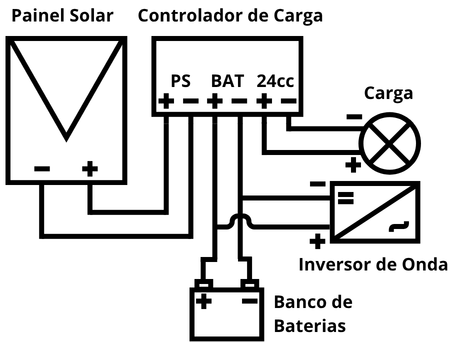
\includegraphics[width=0.50\textwidth]{fig/doc_images/image15}
  \caption{Diagrama simplificado de um sistema Fotovoltaico (FV) \textit{off-grid}.}
  \label{fig:diagrama_fv}
  \fontefig{Fonte: Autoral.}
\end{figure}

Sendo assim, o capítulo a seguir apresenta o detalhamento metodológico empregado no
dimensionamento, na integração e na validação do sistema proposto.
